 Moving on from the discussion of the physics in the ion heat transport model, this chapter describes how the model is encoded as an initial-value time evolution problem, the code structure and boundary conditions, and the diagnostic data used as inputs to the code to predict the evolution of the ion temperature profile throughout the enhanced confinement period of a PPCD discharge. %% Reworded this intro sentence a bit. Please check to see that it covers what you want to say -- MDN 
 %While sizable and important, this is likely one of the least interesting chapters in this thesis. There are no results presented here. (Unnecessary -- MDN)
 The first half of the chapter deals with the diagnostics relevant to this research, their capabilities, and how they are used in the modeling. Then I will discuss the modeling methods and considerations, especially implicit physics assumptions made. Finally I will go over some of the more explicit physics assumptions made as well as boundary conditions and such. 
 % These last two sentences could be much more specific by indicating that the work you are doing is related to ion heat confinement which, for the plasmas densities under study, involves understanding the evolution of the ion temperature over several ms. As such, the relevant time scale is the one on which the equilbrium magnetic pressure varies. The confinement time is 10-15 msec, but since the electrons are heating up during the discharge, the equilibrium evolves during this time. Therefore, although the small-scale dynamics responsible for transport involve much faster fluctuation time scales, the evolution of the equilibrium is well-characterized on the 1 msec (or 500 mircosecond) timescale. All the dynamics faster than this timescale are considered part of the transport physics and parameterized by advection and diffusion coefficients.
 At it's core, this modeling work is a compromise between making it simpler through approximations so that it could be better understood and completed in a reasonable time, but still preserving enough details and grounding in data so that it produces insightful and believable results. In someways, this chapter described and justifies those compromises. 

%===========
%====MST====
\section{A summary of MST and it's diagnostics}\label{sec:MST}
Let's begin with the plasma experiment itself. The Madison Symmetric Torus is a reversed field pinch experiment located in Madison, WI. It was constructed in the 1980s, achieving first plasma in 1988\cite{Dexter1991}. It was designed as a proof of concept device to demonstrate the RFP fusion\cite{Najmabadi1999}. 
% I added this line to put the diagnostics you use in the historical context as well
A number of advanced diagnostics were designed and fielded on the MST as part of a proof of principal program for RFP fusion. %%
The MST is capable of a wide range of plasma conditions and configurations, and improved confinement through current profile control was achieved and refined in the late 1990s\cite{Sarff1995TransportPinch, Chapman2002HighPinch}. This method, referred to as Pulse Parallel Current Drive (PPCD) is a transient process that greatly reduces the tearing mode fluctuations that %plagues
leads to heat transport by stochastization of the magnetic field in
the standard RFP plasma.
To help achieve consistent PPCD plasmas at high currents, the walls are well conditioned, no probes are inserted, and gas puff fueling is carefully timed to preceed the PPCD period. These plasmas are too hot for probe measurements, but instead, a variety of noninvasive advanced diagnostics provide information about the core plasma including interferometry, Thomson scattering measurements, and visible light emission measurements. An array of magnetic pickup coils in the walls provide boundary magnetic measurements. 

\begin{figure}[!htb]
	\centering
	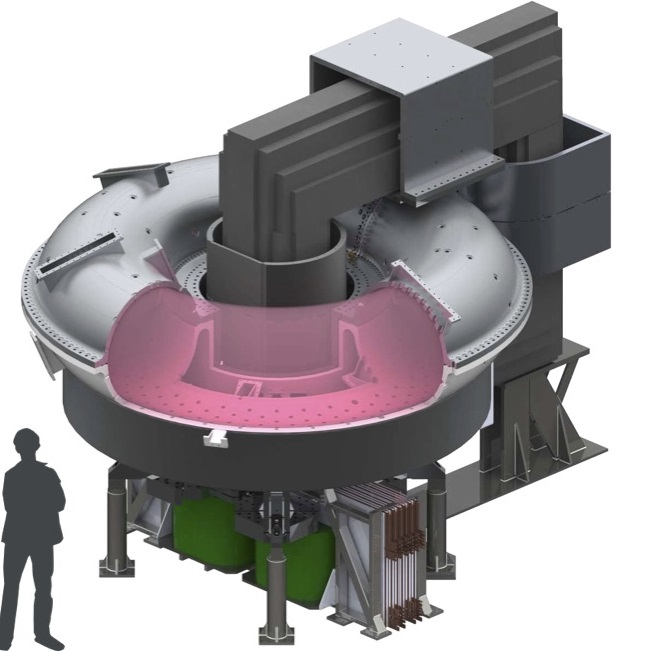
\includegraphics{./implementation/MST_model_diagram}
	\label{fig:MST_diagram}
	\caption[Diagram of MST]{Diagram of MST. Note the close fitting shell, as well as the holes on the bottom of the vessel that lead to the pumping manifold. The pumping duct location will become relevant in section \ref{sec:neutral_dynamics}.}
\end{figure}

\begin{table}[]
    \centering
    \begin{tabular}{||c|c|c||}
        Parameter & MST range & experiment range\\
        \hline
        Major radius ($R$)& 1.5 [m] & -same- \\
        Minor radius ($r$)& 0.52 [m] & -same- \\
        Plasma Current ($I_p$) & 50 ~ 500 [kA] & 480 -500 [kA] \\
        Magnetic Field ($B_t(0)$) & $\leq 0.6$ [T] & $~0.5$/ [T] \\
        Electron Density ($n_e$) & $0.5 - 3 \times 10^{19}$ [$m^{-3}$] & ~$0.7 \times 10^{19}$ [$m^{-3}$]\\
        Electron Temperature* ($T_e$) & 0.05 ~ 1.8 [keV] & 0.9 ~1.5 [keV] \\
        
    \end{tabular}
    \caption[MST parameters]{Basic parameters of MST. The experiment range refers to the parameters of the high current improved confinement plasmas considered as part of this work. }
    \label{tab:my_label}
\end{table}


\begin{figure}[!htb]
	\centering
	\includegraphics{./implementation/MST_diags.PNG}
	\label{fig:MST_diagnostic_diagram}
	\caption[Diagram of diagnostic locations]{A diagram of the MST diagnostics. For PPCD, the toroidal separation of the diagnostic is typically not very important due to the good asymmetry displayed by the plasma. However, for the m=0 burst studies detailed in chapter \ref{ch:m0}, it becomes more relevant. (Reproduced from R. Dexter et al. Ref\cite{Dexter100}}
\end{figure}

MST has a wide range of diagnostics, many of them designed to operate at high data frequencies compared with %to 
%%% ("compared with" is used to contrast while "compared with" is used to identify similarities) -- MDN 
other devices. Ion transport is dependent on a large number of plasma parameters even when only classical effects are considered. Hence, a range of MST's diagnostics are used. The rest of this section aims to give a summary of the principal of operation for the key diagnostics as well as the analysis techniques used to interpret %process (MDN)
the raw diagnostic data. 

%============
%===FIR===
\subsection{Far Infrared Interferometer and Polarimeter}
The Far InfraRed (FIR) interferometer-polarimeter is a laser diagnostic that employs two different physics principles to measure electron density as well as parallel magnetic field strength. While neither measurement directly informs ion transport, they are critical plasma parameters that are needed to calculate the various terms % which terms?
in the model. I will start by giving a short introduction of the two separate physics principles of the interferometer and then that of the parameter. Then I will describe the FIR hardware as available on MST, and finally, I will describe the analysis and incorporation of raw diagnostic data. 

The FIR interferometer relies on the fact that the index of refraction of the plasma is dependent upon the density of the plasma. In short, one laser beam is passed through the plasma, and then compared with a reference beam that passed through air. The relative phase lag is measured by the interferometer and information about the plasma density is extracted. 

To understand this process in more detail, we can begin with a Fourier representation of the electric field of a generic EM wave:
\begin{align}\label{eqn:fir_wave}
    \vec{E}(\vec{x}, t) &= \frac{1}{(2\pi)^4}\int\vec{E}(\vec{k},\omega)e^{i(\vec{k}\cdot\vec{x}-\omega t)}d^3\vec{k}d\omega 
\end{align}
where $\vec{k}$ is the wave vector, and $\omega$ is the angular frequency. The magnetic field component $\vec{B}(\vec{x},t)$ is similarly described.

In a plasma, an EM wave has to further satisfy the wave equation, as well as Ohm's law, which combines into the following:
\begin{align}
    (\vec{k}\vec{k} - k^2\xtensor{\textbf{1}} + \frac{\omega^2}{c^2}\xtensor{\epsilon})\cdot\vec{B} = 0
\end{align}
where $\xtensor{\epsilon} = (1+\frac{i}{\omega\epsilon_0})$ is the isotropic dielectric constant. Taking the cold plasma approximation of $\xtensor{\epsilon}$ and simplifying the result yields the Appleton-Hartree formula\cite{hutchinson_2002},
%%%Also, you use the first-order approximation lower down, so best to solve the relation to first order here.
\begin{align}
    N^2 &= 1 - \frac{X(1-X)}{1-X-\frac{1}{2}Y^2 \sin^2\theta\pm [(\frac{1}{2}Y^2\sin^2\theta)^2 + (1-X)^2Y^2\cos^2\theta]^{\frac{1}{2}}}
\end{align}
where $N$ is the index of refraction, $X = \frac{\omega_p^2}{\omega^2}$ and $Y = \frac{\Omega}{\omega}$. Considering that the cyclotron frequency $\Omega$ is small compared to the FIR laser frequency $\omega$, then $Y \rightarrow 0$. Taking the zeroth-order approximation\cite{Hutchinson_2002},
\begin{align}
N^2 \approx 1 - \frac{\omega_p^2}{\omega^2}
\end{align}
which is only dependent on $n_e$. Under these conditions, measuring the phase difference between a beam that travels through the plasma and a reference beam traveling through the air will give phase difference
\begin{align}
    \Delta\phi &= \int(k_0 - k_{\text{plasma}})dl \nonumber\\
    &= \frac{\omega}{c}\int(N - 1)dl \nonumber \\
    &= 2.814\times10^{-15}\lambda\int n_e dz 
    &\text{\ [For MST conditions]}
\end{align}
The parameter takes advantage of the 1st order approximation of $N^2$,
\begin{align}
    N^2 = 1 - X \pm XY cos \theta
\end{align}
where the addition refers to the ordinary mode and the subtraction refers to the extraordinary mode. The two modes approximately correspond with right and left handed circularized polarization. Given the differing index of refraction for the two circular polarizations, a phase difference results, leading to an effective rotation of initial polarization referred to as Faraday rotation. The rotation angle is given by,
\begin{align}
    \alpha &= \frac{\Delta \phi}{2}\nonumber\\
    &= \frac{1}{2}(N_+ - N_-)\frac{\omega}{c}z \\
    &\approx \frac{e^2 \lambda^2}{8\pi m^2_e c^3 \epsilon_0}\int n_e \vec{B}\cdot d\vec{l} \nonumber \\
    &= 2.62\times10^{-13}\lambda^2\int n_e{\vec{l}}\vec{B}\cdot d\vec{l} &\text{[For MST conditions]}
\end{align}

\begin{figure}[!htb]
	\centering
	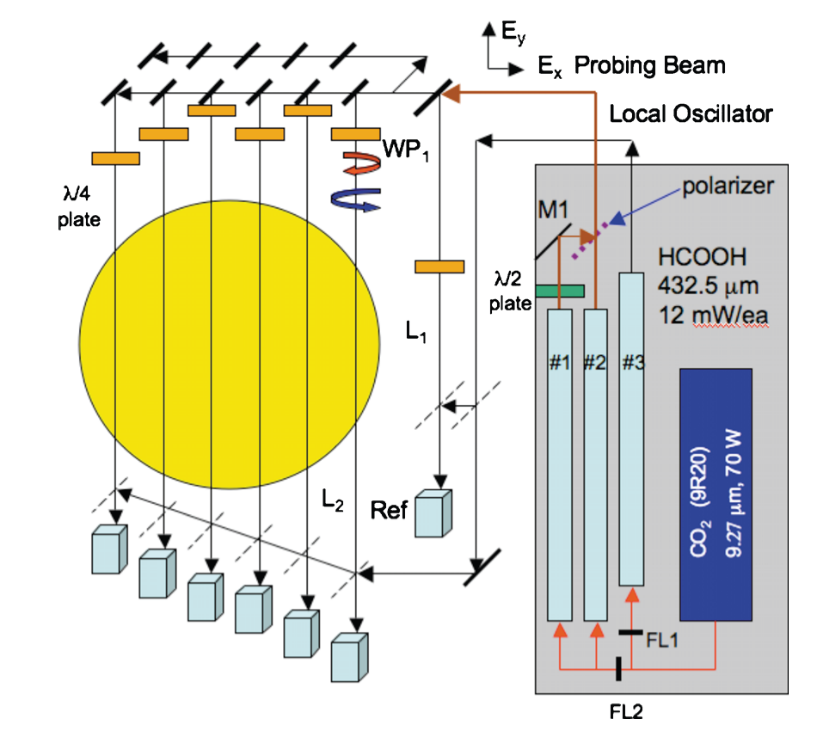
\includegraphics[width = 0.9\linewidth]{./implementation/fir_optics_diagram.PNG}
	\caption[Diagram of FIR optical paths]{Diagram of FIR system optical paths. Lasers marked \#1 and \#2 are orthogonally polarized for polarimetry measurements, and laser \#3 is used as the `local oscillator' necessary for heterodyne phase detection for the interferometry measurements. (Reproduced from E. Parke, et al.\cite{Parke2016})}
    \label{fig:fir_optics_diagram} 
\end{figure}

MST's FIR system consist of a CO$_2$ laser pumping three formic acid cavities in a heterodyne system. The three formic acid cavities are pumped using the same CO$_2$ laser in order to reduce the effects of power fluctuation on the output beam since all three beams are proportional to the pump power. The CO$_2$ pumping laser is a commercially available model with a tunable laser cavity allowing it to be tuned to the FIR pumping frequency. The formic acid laser cavities are custom built and can be tuned independently via motor mounted mirrors. The formic acid lasers convert the ~$10\mu m$ photons from the CO$_2$ laser to ~$432.5\mu m$ (~700GHz) for the probing beams. To facilitate heterodyne detection of phase, the formic acid lasers are further tuned to relative frequencies on the order of 1 MHz. The optical system splits the probing beam into 11 independent measurement chords, as well as separate reference and 'local oscillator' beams paths using thin wire mesh beam splitters. Figure \ref{fig:fir_optics_diagram} provides an illustration of the optical setup. The laser beams, after completing their designated path, are measured with recently installed planar-diode mixers at 6 Mhz. These mixers have high sensitivity and reduced noise floor allowing fluctuation measurements of up to 250 kHz for polarimetry and 600 kHz for interferometry\cite{Parke2016}. 
\begin{figure}[!htb]
	\centering
	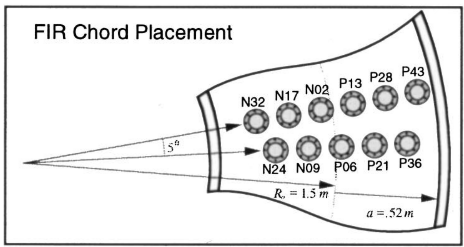
\includegraphics[width = 0.75\linewidth]{./implementation/fir_chords.PNG}

	\caption[Diagram of FIR chord offset]{Diagram of FIR system's 11 viewing chords separated into 2 sets, 5\textdegree\ apart. (Reproduced from N. Lanier, et al.\cite{Lanier2001}}	
	\label{fig:fir_chords}
\end{figure}

The 11 measurement chords are further separated into two sets, about $5\degree$ toroidally separated from each other (see figure \ref{fig:fir_chords}). This has been taken advantages of to make toroidal fluctuation measurements, but for the purpose of the PPCD plasmas investigated in this work, only their radial locations are considered. 

It is pertinent to note that the electron density profile is not determined from a simple inversion of FIR interferometry measurements, but rather incorporated as constraints with other diagnostics measurements in a Grad-Shafranov equilibrium calculation \cite{Anderson2001} as discussed in more detail in section \ref{sec:MSTfit}.

%==D_alpha==
\subsection{The $D_{\alpha}$ array}\label{sec:dalpha_array}

Neutral particle density profiles are determined by modelling the neutral particle dynamics from particle sources and sinks which are constrained by the measurement of deuterium Balmer-alpha (or $D_{\alpha}$) emissions arising from the $n=3$ to $n=2$ transition. $D_{\alpha}$ emission occurs when a deuterium atom is excited to a higher state, usually through electron impact excitation or charge exchange. The associated radiance can be calculated as,
\begin{align}
    R &= \int_C \frac{\Delta \Omega(\vec{r})}{4\pi}\gamma_{D_{alpha}}(\vec{r}) dl\\
    \gamma_{D_{alpha}} &= \frac{A_{32}}{ A_{32} + A_{31} }\left( n_0 n_e <\sigma v>_{\text{excitation}} + n_0 n_i <\sigma v>_{\text{CX}} \right)
\end{align}
% You call this quantity "the rate of photon generation," but a check of the units shows that it has units of m^-3/s. I suspect that this is the number of photons produced per volume. The usual radiometric quantity to report here is the "radiance" which has units of Watts/(m^2 Sr). This is the amount of radiant energy emitted from a surface per solid angle per time. It may make sense to write this quantity out in terms of the line-integrated emission coefficient (units of W/(m^3 Sr)) since this is what you are measuring and forward-modelling in DEGAS2.
%--
%Changed, although what DEGAS2 does is much more complicated than this integral as it uses sub-chords and calculating percent contribution of a finite volume and so on. The complications is partly why I chose originally to present the photon generation per volume per time calculation. --Xing
where $n_0$ is the neutral density, and $<\sigma v>$ are the distribution averaged reaction rates for electron impact excitation and charge exchange into the neutral deuterium $n=3$ excited state and $A_{32}$ and $A_{31}$ are the Einstein coefficients for spontaneous emission. Given $n_e$, $n_i$, and $n_0$ the neutral emission is easy to calculate, but it varies over $3$ orders of magnitude across the plasma diameter with very little emission arising from the hot core. Accurately determining the neutral density in the core requires careful calculations of the neutral dynamics which are discussed in detail in section \ref{sec:DEGAS2}.


\begin{figure}[!htb]
	\centering
	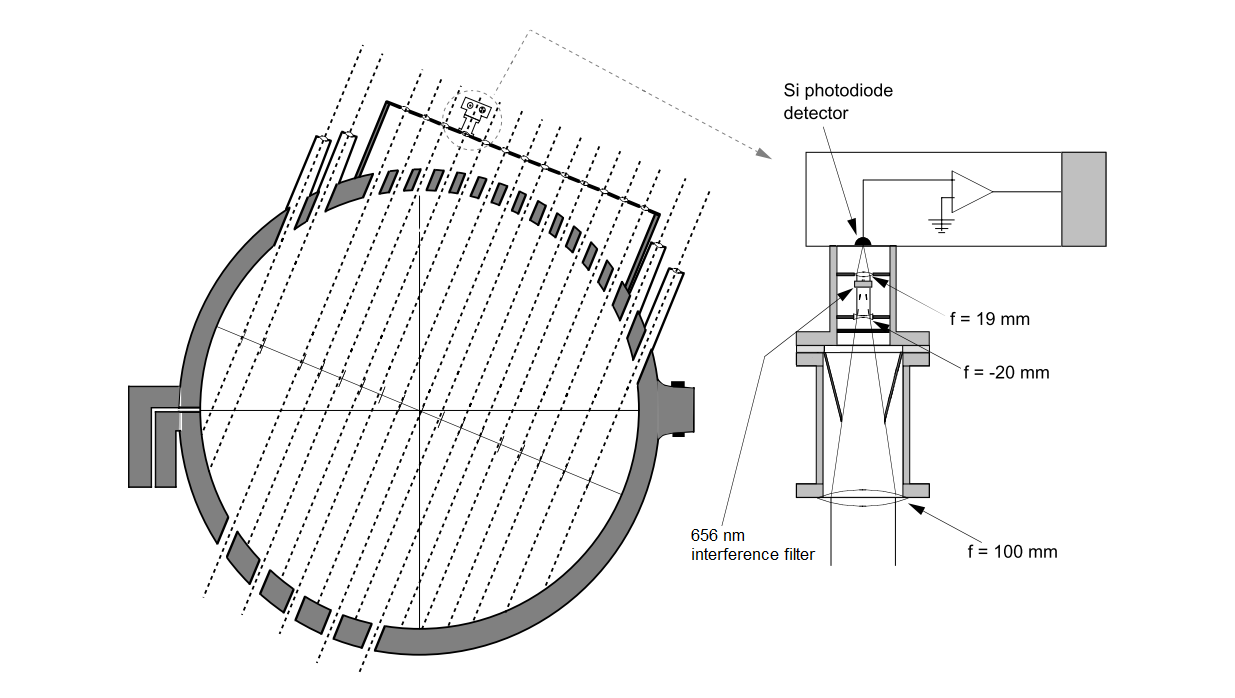
\includegraphics[width = 0.9\linewidth]{./implementation/d_alpha_detector.PNG}
	\caption[$D_{\alpha}$ detectors]{Diagram $D_{\alpha}$ detectors and available viewing chords. The detectors consist of focusing optics, a silicon photo-diode, and a trans-amplifier circuit. In some detectors there is also a pin-hole aperture used to reduce the intensity of incident light on the detector. Five of the viewing cords have matching ports on the other side, but they are not used for this work. (Reproduced with modifications from J. Anderson\cite{Anderson2001})}
	\label{fig:D_alpha_diagram}
\end{figure}

MST uses 13 silicon photo-diode detectors to observe the 656nm $D_\alpha$ line.  The detector array (referred to as the $D_{\alpha}$ array) is located at the $210 \degree$ toroidal boxport. The boxport has 17 available lines of sight, hence we are limited by the avaliable detectors. The detectors consist of filtered silicon photo diodes with a built-in current-to-voltage transimpedance amplifier. Figure \ref{fig:D_alpha_diagram} shows the physical assembly of the detectors.

\begin{figure}[!htb]
	\centering
	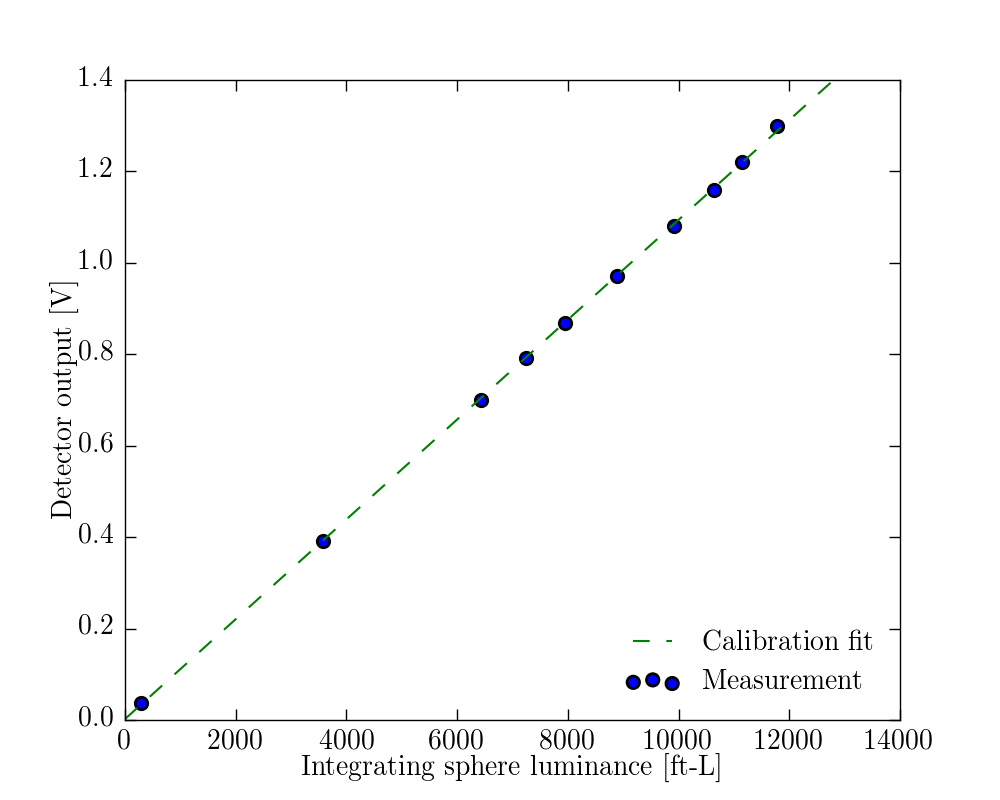
\includegraphics[width = 0.9\linewidth]{./implementation/diagnostics/l_vs_v.png}
	\caption[Example $D_{\alpha}$ calibration]{Example voltage vs luminance calibration for $D_{\alpha}$ detectors. This in particular is from detector \#32's calibration from Aug. 2015.}
	\label{fig:l_vs_v}
\end{figure}

The detectors are calibrated using a commercially available Tungsten strip-lamp with integrating sphere which has been calibrated for radiance measurements. An optical assembly identical to that on MST is used to couple light from the integrating sphere to the detector. Since the optical geometry is reproduced, the geometrical effects quantified by the {\'e}tendu $A\Delta\Omega$ are held to be constant between calibration and machine. However, the transfer function is much wider than the $H_{\alpha}$ emission line, and thus needs to be taken into account. Namely the voltage measured in calibration is
\begin{align}
    V_{\text{cal}} &= c A \Delta\Omega \int^{\infty}_{0}f(\lambda)R_\lambda(\lambda)\ d\lambda\\
    &\equiv c'R
\end{align}
where $c$ and $c'$ are calibration factors, $f(\lambda)$ is the transfer function of filter, and $R_\lambda$ is the spectral radiance of the integrating sphere. With $c'$ thus defined, it can be easily calculated from measured pairs of output voltage {\em vs} luminance slope from,
\begin{align}
    c' &= \frac{V_{\text{cal}}}{R}\\
    &= \frac{\Delta V}{\Delta L}\left(\frac{L}{R}\right)_{\lambda}
\end{align}
where $\frac{\Delta V}{\Delta L}$ is the measured voltage vs. luminance slope (see Figure \ref{fig:l_vs_v}), and $(\frac{L}{R})_{\lambda}$ is the luminance to spectral radiance conversion factor provided by NIST-certified calibration of the light source. To apply to measurements, however, we have to further consider that the voltage due to measurement of plasma emission is
\begin{align}
    V_{\text{meas}} &= c A\Delta\Omega\int^{\infty}_0\int_{C} f(\lambda)\epsilon(\lambda,l)\ dld\lambda
\end{align}
where C is the view path, l is the distance along the line-of-sight, and $\epsilon$ is the spectral emissivity. Since the plasma emission is a discrete emission line and the calibrated light source is a broad-spectrum source, we cannot equate the integration over spectral wavelength between the calibration and plasma measurements. Thus, an additional factor is needed. Approximating the spectral emissivity as a delta function, {\em i.e.} $\epsilon\approx I_{D_{\alpha}}(l)\delta(\lambda - \lambda_{D_{\alpha}})$ where $I_{D_\alpha}$ is the emissivity, the measured voltage becomes
\begin{align}
    V_{\text{meas}} &= c A\Delta\Omega f(\lambda_{D_{\alpha}}) \int_{C}I_{D_{\alpha}}(l)\ dl \nonumber\\
    &= c' \frac{f(\lambda_{D_{\alpha}})}{\int_0^{\infty}f(\lambda)d\lambda}\int_C I_{\dal}(l)\ dl \\
    &\equiv c' c_{\text{trans}}\int_C I_{\dal}(l)\ dl 
\end{align}
where in addition of the calibration factor $c'$ defined previously, the transfer function normalization factor $c_{\text{trans}} \equiv \frac{f(\lambda_{D_{\alpha}})}{\int_0^{\infty}f(\lambda)d\lambda}$ is also need for the proper calculation of the line emission intensity. This latter factor $c_{\text{trans}}$ was precisely measured using a high-resolution Ocean Optics HR2000+ spectrometer as the transfer function of the filters showed noticeable variations\cite{Eilerman}, but it is not regularly re-calibrated as it would require disassembly of the detectors. The radiance calibration of $c'$ using the integrating sphere is performed once a year during the data taking period for this work. More details of the hardware and calibration process can be found in Anderson's Ph.D. thesis\cite{Anderson2001} (Chapter 2) and Eilerman's Ph.D. thesis\cite{Eilerman} (Appendix A).


\subsection{The Thomson Scattering Diagnostic}

The Thomson Scattering (TS) diagnostic is a laser-based optical diagnostic which operates via the eponymous Thomson scattering process. On MST, it is setup to provide $T_e$ measurement, though the physics of the Thomson scattering process is in theory able to provide both temperature and density information about either electrons or ions. Thomson scattering itself can be understood as the limit of Compton scattering of photons on free charged particles at the limit of low photon energy, in this case, free electrons in the plasma. In short, the free electron will scatter incident photons to a new direction while preserving frequency. But individual electrons travels at various speeds and directions and will thus encounter variously blue and red shifted incident photons from the laser, causing the scattered output to experience line broadening analogous to Doppler broadening. In particular, the TS diagnostic takes advantage of incoherence (or non-collective) Thomson scattering in the plasma.  In this case, the wavelength of the incident photons are much smaller than the Debye length of the plasma, thus the plasma will not respond collectively to the light, but instead electrons respond approximately individually. The mechanics of Thomson scattering is best explained in the classical wave-based picture. The incident E-M wave accelerates free electrons in a oscillatory fashion, and as an oscillating charge, the electron radiates E-M waves in all directions with the same frequency with an intensity pattern that varies with the incident angle. In a plasma context, a powerful laser is used to provide the incident light at a specific frequency, and the scattered light is observed. However, the scattered light from a plasma is not the work of a particular electron, but made up from many individual scattering events off of many electrons. The electrons have a distribution of velocities in the direction of the incident beam, and as mentioned above, scatters the incident beam over a distribution of wavelengths. Thus, the intensity of the scattered light from a plasma is a function of scattering angle, electron density, as well as electron temperature. This intensity function is further modified due to relativistic effects important for hot plasmas ($>1$ keV). 
 
The spectral intensity $S(\epsilon, \theta, \alpha)$ (the directed scattered power per solid angle per normalized  wavelength shift $\epsilon$) due to scattering by a Maxwellian distribution of electrons are first calculated by Zhuravlev and Petrov\cite{Zhuravlev1979} and expanded upon by Seldon\cite{Seldon1980} for routine analysis as follows:
\begin{align}
    S(\epsilon, \theta, \alpha) &= \frac{c(\alpha)}{A(\epsilon, \theta)}e^{-2\alpha B(\epsilon,\theta)} \label{eq:Sheldon}\\
    &\text{where:}\nonumber\\
    A (\epsilon, \theta) &= (1+\epsilon)^2\sqrt{1(1- \cos\theta)(1+\epsilon) + \epsilon^2} \nonumber\\
    B (\epsilon, \theta) &= \sqrt{1 + \frac{\epsilon^2}{2(1-\cos\theta)(1+\epsilon)}} - 1 \nonumber\\
    c (\alpha) &= \sqrt{\frac{\alpha}{\pi}}(1 - \frac{15}{16}\alpha^{-1} + \frac{345}{512}\alpha^{-2} + \ldots) &\text{for } \alpha \gg 1 \nonumber
\end{align}
and $\alpha \equiv \frac{1}{2}\frac{m_ec^2}{kT_e}$, $\epsilon = \frac{\lambda_s}{\lambda_i}$ is the normalized wavelength shift, and $\theta$ is the scatter angle. This analytical calculation does not account for depolarization effects, but observations have shown that for the characteristic parameters of MST, the depolarization effects can be safely ignored\cite{Seldon1982}. 

\begin{figure}[!htb]
	\centering
	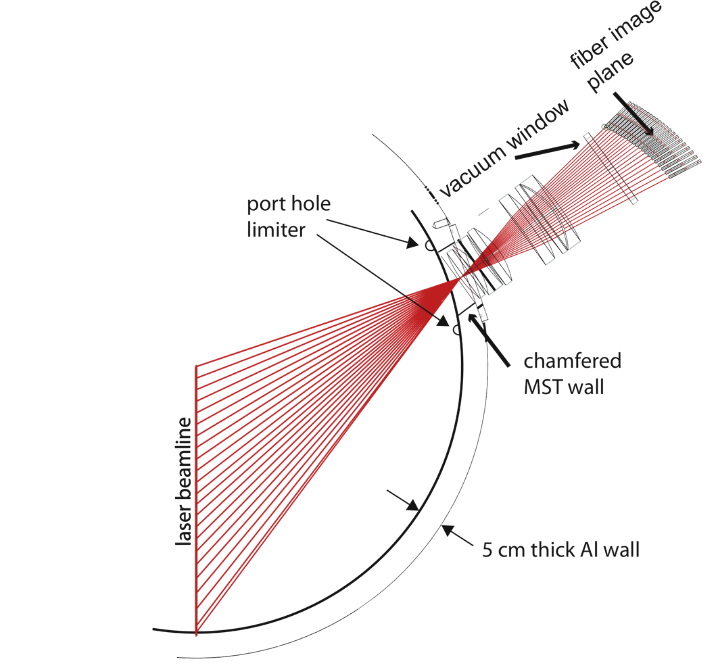
\includegraphics[width = 0.9\linewidth]{./implementation/diagnostics/ts_optics_diagram.png}
	\label{fig:ts_optics_diagram}
	\caption[Diagram of Thomson scattering optics and sight lines]{Diagram of Thomson scattering optics and sight lines. The scattering angle in equation \ref{eq:Sheldon} are dictated by angle made by the red view paths and the laser beam line. (Reproduced from J. Reusch.\cite{Reusch2011})}
\end{figure}

In MST, the TS diagnostic has 21 sight-lines. The scattering angle for a particular sight-line is fixed by the geometry of the viewing optics and ranges from $\sim 108\degree$ to $\sim 143\degree$. The wavelength dependence is observed via an array of polychromators equipped with avalanche photo-diodes digitized at 100MHz to help separate the scattered laser light from the background (digitized both before and after the laser pulse). The temperature $T_e$ is found via least \chisq\ fitting of these observations. The temperature measurements are localized by the intersection of the laser beam path and the viewing geometry, allowing direct $T_e$ profile measurements without relying on inversion techniques. The main limiting factor of TS diagnostics are the fact very little of the incident beam power is scattered (ie. the cross section is very small), and thus it relies on a very powerful pulsed laser (pulse energies $\sim$ Joule) to provide the incident beam. Such lasers are often limited in their repetition rate due to the technical difficulties with heat in the lasing medium, thereby limiting the ability to diagnose fast phenomenon. MST's TS system is powered by two laser ``backends.'' The older ``work-horse'' system is based on a pair of off-the-shelf Q-switching Nd:YAG lasers operating at 1064nm. A series of upgrades have been made to the Pockel cell drivers (that are responsible for Q-switching) and power supplies that significantly increase the repetition rate achieved to up to $\sim 1$~kHz per laser over $\sim 15$~ms of active time\cite{DenHartog2010}. In standard operation, the two lasers' timing are staggered in such a way to achieve effectively a 2~kHz pulse rate. This is the mode used to take the data related to this research, as it focuses more on the slower time scale effects the electron $T_e$ have on the ions. The effective TS frequency of 2~kHz affects the rate at which the plasma kinetic profiles are updated and sets the evolution timescale of the model. This issue will be addressed in more detail in section \ref{sec:time_blocks_and_steps}. For studies of faster plasma phenomenon, the Spectron lasers can also be operated in a pulse-burst mode\cite{DenHartog2010} where bursts very fast pulses are produced and repeated. A typical repetition rate in this mode produces 8 pulses at 25~kHz, and these bursts themselves repeats at 1~kHz. The TS system also has an alternative custom-built laser system commonly called the Fast Thomson system despite the fact that the `regular' TS system is already very fast. The Fast Thomson system can be operated at a repetition rate of up to 333~kHz for 3-4 pulses, or 100~kHz for 44 pulses\cite{Young2015}, giving it exceptional capabilities to resolve fast $T_e$ dynamics. It is, however, not relevant this this work. 

A detailed overview of MST's TS system can be found in the thesis of J. Reusch\cite{Reusch2011}, and an recent comprehensive treatment of TS theory is available by Prunty\cite{Prunty2014}.


\subsection{Ion Doppler and charge exchange recombination spectroscopy}\label{sec:ids}

Naturally occurring ion line emission in the plasma due to electron impact excitation and charge exchange with recycled neutral deuterium, is shifted in wavelength by ion velocity due to the Doppler effect and broadened due to the the thermal velocity distribution of the plasma ions. The broadening occurs since a portion of the observed line emission is red-shifted due to ions having velocity away from the observer and an portion is similarly blue-shifted. A net flow velocity in the plasma causes a net wavelength shift. Spectrally resolved measurements of this line emission can be observed using a spectrometer to determine the emitting ion population's density, velocity, and temperature.

\subsubsection{Physics principles of IDS}
The emission lines used to make theses observations can come from one of three reactions: electron impact excitation, charge exchange recombination, or radiative recombination. For the range of plasma temperature and density achieved in MST, %and in fusion physics in general, (This is not true for a detached diverter for example)
the radiative recombination is a negligible contribution. Typical line emission from MST consist primarily of the result of electron impact excitation and neutral deuterium charge exchange reactions with impurities. The impurities themselves are either atmospheric contaminants (like oxygen) or sourced from limiter sublimation (carbon) and wall sputtering (aluminum). Since this line emission is naturally occurring in the plasma, only a spectrometer and appropriate viewing optics are necessary to observe the emission to obtain information about the plasma. But ion Doppler spectroscopy using naturally-emitted line emission integrates light emitted from the entire plasma volume along the line of sight which is typically not uniform. This means the measurements are not localized except by the emission shells that form for partially-ionized ions in the temperature gradient regions of the plasma. Interpreting this emission requires detailed calculations of ion charge state which depends on the electron temperature and density as well as the neutral deuterium density and it can be a challenge to interpret measurements made. 

Charge exchange recombination spectroscopy (CHERS, or CER) is a special case of Doppler spectroscopy where a neutral beam is used to stimulate charge exchange emission along its path, allowing the spectrometer to make localized measurements where the beam and line of sight intersects. The Doppler shift due to the line-of-sight velocity of an emitting ion is 
\begin{align}
    \Delta\lambda = \lambda_0 \frac{v}{c}.
\end{align}
If we assume a Maxwellian distribution of emitting ions, then the lineshape of the spectral radiance is 
%altered from the $R(\lambda) = I_0\delta(\lambda_0)$ to 
% Technically, there is always some broadening, no matter how small. Even for very cold ions in atomic traps there is broadening due to quantum mechanical uncertainty effects referred to as "natural broadening."
%--
%Got it. -Xing
\begin{align}
    R(\lambda | v, T, I_0) &= \frac{I_0}{\sigma_\text{th} \sqrt{2\pi}}I_0 e^{\frac{-(\lambda-\lambda_c)}{2\sigma_\text{th}^2}}\\
    &\text{where:}\\
    I_0 &= n_{\text{imp}}n_s \left< \sigma v \right>^* &\text{is the total intensity}\\
    \sigma_\text{th} &= \frac{\lambda_0}{c}\sqrt{\frac{kT_\text{imp}}{m_{\text{imp}}}} &\text{is the thermal broadening, and}\\
    \lambda_c &= \lambda_0(1+\frac{\left< v_\text{imp} \right>}{c}) &\text{is the velocity shifted wavelength.}
\end{align}
Additionally, $n_s$ is the density and $\left<\sigma v\right>$ is the effective reaction rate (with branching fraction modification) of the emission generating reaction, $T_\text{imp}$, $<v_\text{imp}$, and $m_\text{imp}$ are the impurity temperature, velocity, and mass. This equation only considers thermal broadening of the line emission. One advantage that can be seen from this formula is the fact that the 3 plasma parameters of interest can be separated easily for analysis. For example, this thesis uses Doppler spectroscopy to look at impurity temperature, thus absolute calibration of wavelength is unimportant for this work as it effective folds into the $\lambda_c$ parameter. In general, the temperature corresponds to width, velocity to total shift, and density to the integrated radiance. 

Modelling charge exchange requires a bit of special consideration regarding both the isolation of the charge exchange emission, as well as the effect of fine structure broadening. To start, the charge exchange emission observed is contaminated by the same emission line excited through electron impact, referred to as background emission. To extract the local plasma information from the charge exchange emissions, the spectrometer also needs a 'reference' sight-line that looks at (effectively) the same plasma but in the absence of the beam. On MST this is done by having a second parallel sight-line offset about 2~cm toroidally. This way, the background emission can be fitted to a spectrum model and then incorporated into the combined charge exchange and background model for the measurements' sight-line. The second consideration has to do with fine structure of the emission line itself. Ultimately, line emission is the result of a bound electron dropping from one energy state to another and emitting a photon of energy equal to the difference of the energy levels. The energy states associated with primary quantum number $n$ consist of sub-levels due to the interaction of the electron orbital angular momentum with the spin angular momentum. The quantization of the angular momentum introduces the other quantum numbers, $l$, and $s$. Each of the energy sub-levels is also Doppler broadened effectively turning the line emission spectrum into the sum of many Gaussians, known as fine structure. The sub-levels associated with the spin number $s$, is due to Zeeman splitting, and the energy effect is small due to the relatively low magnetic field, and is not significant for the broadening calculations. The angular quantum number $l$ and the energy sub-levels associated have a significant effect on emissions, and charge exchange emissions especially.  Then, it is important to know the relative wave lengths and amplitudes of these component Gaussian emissions. But these can be difficult to calculate analytically as the probability of populating a certain fine structure level is complex and has many dependencies. These calculations have been performed elsewhere\cite{Isler1994}, this thesis instead relies on the Atomic Data and Analysis Structure (ADAS) database for the relative population of the fine structure states\cite{Summers2004}. 

\begin{figure}[!htb]
	\centering
    \begin{subfigure}[t]{0.5\textwidth}
        \centering
        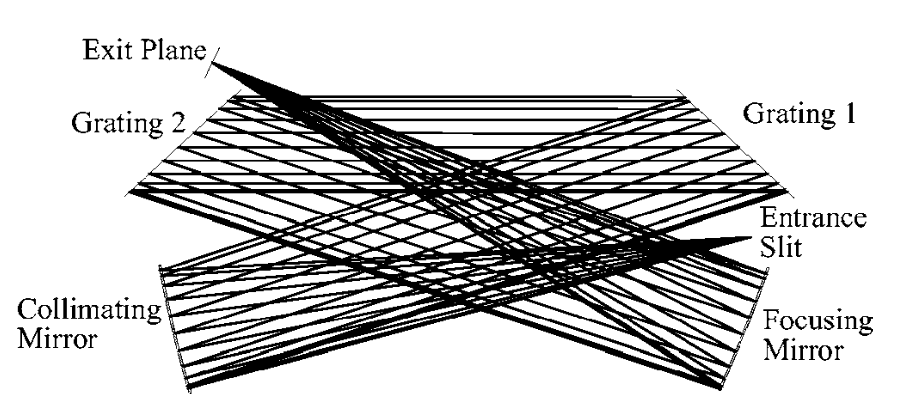
\includegraphics[width = \textwidth]{implementation/diagnostics/idsii_trace.png}
        \caption{Optical layout of IDS-II via ZEMAX}
    \end{subfigure}%
    ~ 
    \begin{subfigure}[t]{0.5\textwidth}
        \centering
        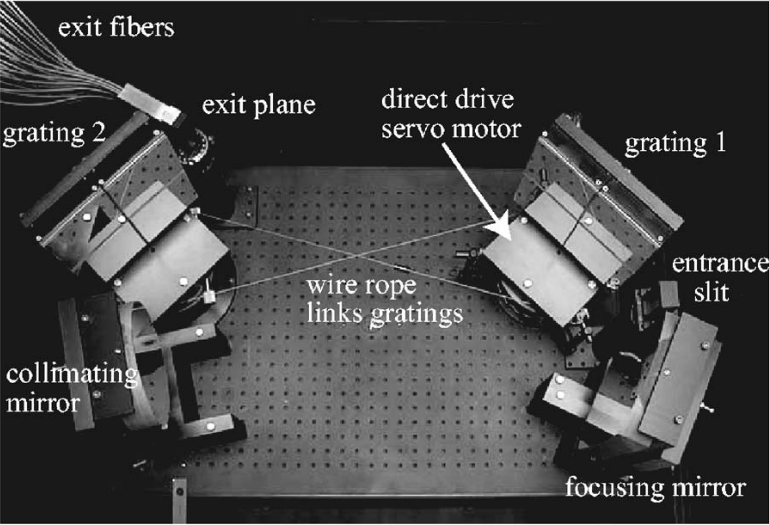
\includegraphics[width = \textwidth]{implementation/diagnostics/idsii_photo.png}
        \caption{Photograph of IDS-II layout}
    \end{subfigure}
	\caption[IDS-II optical layout]{IDS-II optical layout. Reproduced from Craig et al. \cite{Craig}}
	\label{fig:IDS-II}
\end{figure}

\subsubsection{Doppler spectroscopy hardware on MST}
On MST, ion Doppler spectroscopy is performed using the IDS-II (ion Doppler spectrometer, mkII). It is a custom built, high throughput spectrometer optimized for the 343~nm C~VI line, but it could be used for any viable emission line between 200~nm and 480~nm. This spectrometer can simultaneously measure emission from light collected along two optical views, either for the measurement and the reference views used for Charge exchange recombination spectroscopy, or two passive Doppler spectroscopy locations simultaneously. It uses a double grating Czerney-Turner design to achieve a high resolving power ($\lambda/\Delta\lambda \sim 5600$) while each of the gratings are actually a mosaic of 4 gratings, giving an large total area in order to achieve the high {\'e}tendu of 0.40 mm$^2$sr per view(see figure \ref{fig:IDS-II}). It uses a series of photo-multiplier tubes (PMTs) to measure the spectral radiance, allowing the system to achieve an effective data rate of up to 100~kHz in high current plasmas\cite{Craig}. Recent improvements improvements to the frequency response of the transimpedance-amplifiers have allowed fluctuation measurements up to 400~kHz\cite{Nishizawa2016}.


\begin{table}[h!]
    \centering
    \begin{tabular}{||c|c|c||}
        Chord \# & r/a & $\rho_v/a$\\
        \hline 
        1 & -0.91 & -0.92 \\
        2 & -0.76 & -0.80 \\
        3 & -0.58 & -0.64 \\
        4 & -0.41 & -0.48 \\
        5 & -0.24 & -0.32 \\
        6 & -0.07 & -0.15 \\
        7 & 0.11 & 0.03 \\
        8 & 0.28 & 0.20 \\
        9 & 0.45 & 0.37 \\
        10 & 0.62 & 0.55 \\
        11 & 0.80 & 0.75
        
    \end{tabular}
    \caption[IDS-II view chord locations]{IDS-II poloidal viewing chord locations. The $\rho/a$ refers to average magnetic flux surface location in axisymetric plasmas.}
    \label{tab:ids_chord_loc}
\end{table}

The IDS-II system has 11 poloidal viewing chords available, listed in table \ref{tab:ids_chord_loc}. It also has toroidal views available, but they are not used for this project since over the time scales studied the ion temperature is isotropic. 

A diagnostic neutral beam (DNB) is used to inject neutral particles to make localized CHERS measurements. The 'diagnostic' in it's name refer to the fact that the beam current is small such that it does not effectively perturb the plasma being observed, in comparison with heating and fueling beams that are designed to increase the temperature and density of the plasma. The DNB on MST is a nominally 50 ~keV, 4~A hydrogen neutral beam with a pulse length of 20~ms\cite{Feng2016}. The beam energy is optimized for the C$^{6+}$ charge exchange emissions which has a peak reaction rate at 45-50~keV. The beam has recently undergone a refit and the beam composition is measured to be about 75\% at full energy, 20\% at half energy and 5\% at a third energy.\cite{Feng2016}

\subsubsection{Line fitting and ensemble analysis}

This work uses the CHERS data obtained in two different modes and a brief discussion of the line fitting and ensembling techniques is needed to place them in context. The raw signals from the PMTs are digitized at 1MHz, but as discussed above, the spectrometer is designed for data-rates up to 100kHz; the difference is account for in the analysis algorithm. A linearized fluctuation analysis technique alternative to the one described here has been developed to analyze fluctuations up to 400kHz\cite{Nishizawa2017}, however this work focuses on the slower dynamics of the quai-equilibrium values and does not use this alternative. The default method starts by converting the 1MHz data into intensity through gain calibration values, then they are summed into time bins at the desired data frequency (1kHz to 100kHz are common), and subsequently, its photon-counting uncertainty is calculated from calibration (described in detail in T. Nishizawa's thesis\cite{Nishizawa2018}). Afterwards, a piece of code calculates the intensity that each PMT channel 'should' measure at a given temperature, velocity, and amplitude, but also accounting for fine structure and instrumental transfer function. A \chisq value is calculated from this model and the actual measurement, and a nonlinear optimization function is used to find the parameters at which the \chisq\ is minimized. If data analyzed is from two passive IDS views, they are fitted independently the same way. However, if a CHERS measurement is being analyzed, then the passive view (the reference) is analyzed as above, and the active view analysis incorporates this result. It does this by adding the passive contribution to the modeled intensity used to calculate the \chisq\ for the active view. Note that the fine structure for the passive emission and the active can be different as they are difference processes, but the instrumental transfer function are dependent on the view not the process. With this addition, the \chisq\ for the active channel is minimized and the analysis complete.

%%Hey Mark, this section below is going to change significantly, possibly disappear. 
Ensembling of data across multiple shots are used to improve the uncertainty of the measurements. The uncertainty for a particular fit is calculated using the co-variance of the \chisq as a function of the fitting parameters. In effect evaluating the 'width' of the \chisq well in each dimension. If the plasma conditions are perfectly repeatable within the ensembled shots, then the uncertainty of the ensemble can be calculated as the uncertainty of the mean, ie. $\sigma_{\text{ens}} = \frac{\Sigma \sigma}{\sqrt{N}}$. However, the shot to shot variation is not insignificant and the total uncertainty presented is $\sigma_{\text{ens}} = \sqrt{ (\frac{\Sigma \sigma}{\sqrt{N}})^2 + \sigma_{\text{shot to shot}}^2}$, and the shot to shot variation is characterized by the standard deviation of the average ion temperature during the PPCD period of each shot in the ensemble.

This method of uncertainty estimation is appropriate for the relatively slow 10kHz fits used for the model comparison work. However, the m = 0 burst analysis presented in chapter \ref{ch:m0} uses fast 50kHz fits, ensembled over m = 0 burst events. The shorter integration time used for the faster fitting means that each fits are noisy enough that sometimes the \chisq 'well' is poorly formed. Also, the burst to burst variation can be large and changes over the burst period. Hence, the uncertainty on the bursts are presented using the upper and lower values that bounds a 67.8\% of the points in the ensemble (\textit{i.e.} 1 sigma). This is chosen instead of the standard deviation value during the burst itself, the distribution of temperature values of a particular ensembled 'bin' tends to be skewed. 
